\section{Isolation Forest}
\label{sec:IsolationForest}

Similarly to the Random Forest, which is used for classification, the Isolation Forest is an ensemble method that is used for anomaly detection. The idea is to train the decision trees to isolate the data from each other, rather than profiling the normal data, and then provide a score that represents how isolated the data is. The more isolated the data is, the more likely it is to be an anomaly. This algorithm was introduced in 2008 by \cite{iforest}, the paper also provides a way of computing the anomaly score.

This algorithm has the advantage of being very fast to train and requiring very little memory. For hour purposes, as previously said, it is more important to have an algorithm that is fast to evaluate a new instance, than an algorithm that is fast to train.

\subsection{Training}
The algorithm is available in \texttt{sklearn} library, and it is very easy to use. This is a truly unsupervised algorithm, the function only takes the dataset as input and manages to automatically select all the rest of the parameters. As an example, I used the same dataset used in the previous sections for the \gls{dbscan} and {\gls{gmm}} algorithms. The result is shown in \autoref{fig:IsolationForest}.

\begin{figure}
    \centering
    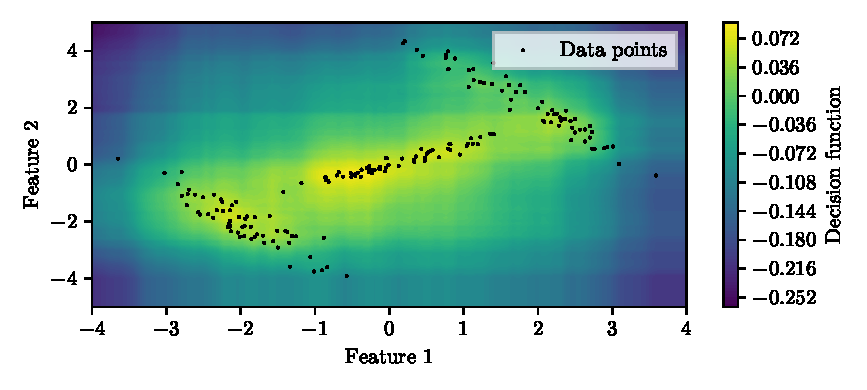
\includegraphics{images/IForest/Figure_1.pdf}
    \caption{Isolation Forest decision function.}
    \label{fig:IsolationForest}
\end{figure}

\subsection{Evaluation of a new instance}
\label{sec:iforest_eval}
The implementation in \texttt{sklearn} provides a function called \texttt{decision\_function}, plotted as a heatmap in \autoref{fig:IsolationForest}. the higher the value, the more likely it is to be a normal instance.
To maintain coherence with the work done up to now, we can take the negative value of \texttt{decision\_function} as a metric to evaluate the novelty of a new instance.

\subsubsection{Selecting the threshold}
\label{sec:iforest_threshold}
With this algorithm is it difficult to geometrically interpret the decision function, so it is not possible to select the threshold a priori. The approach could be to look at the values of the decision function on the training dataset and select a value slightly higher than the maximum value for the training dataset.

\subsection{Limitations of Isolation Forest}
The main limitation is that since the algorithm is based on decision trees, the decision thresholds are defined on the features axis, so the decision boundaries are highly dependent on the alignment of clusters with the axis. looking back to \autoref{fig:IsolationForest}, we can see that the decision function has roughly the same value in the lower right corner as in the lower left corner, even if the lower right corner is clearly more isolated than the lower left corner. This is because the decision boundaries are aligned with the axis, and the lower right corner is more isolated only in the diagonal direction.

The complexity of the training phase is $\mathcal{O}(t\psi\log\psi)$ where $t$ is the number of trees used, and $\psi$ is the size of the subsampling size. The complexity of the evaluation is instead $\mathcal{O}(t\log\psi)$ \cite{iforest}.